\section{rSLA DSL}
\label{sec:dsl}
alphabet, vocabulary, language structure

production rules


\subsection{rSLA language structure, alphabet}

 point of this subsection?

The rSLA language follows the semantic decomposition of the WSLA specification \cite{wsla}, where an SLA takes the form of a hierarchical tree with a 
single root node and numerous uni-directional edges. Figure \ref{rSLA_diag} illustrates the rSLA vocabulary as a tree of classes that the rSLA DSL 
implements. Connections between nodes in the rSLA tree highlight the nesting of SLA context. 

In the rSLA alphabet the root node of an rSLA tree represents an SLA object. In Figure \ref{rSLA_diag} nodes that are positioned close to the root, 
designate branches of SLA context (e.g. base and composite metrics, service level objectives). Edges between nodes are uni-directed to illustrate the 
rSLA tree hierarchical schema.

\begin{figure}
  \centering
    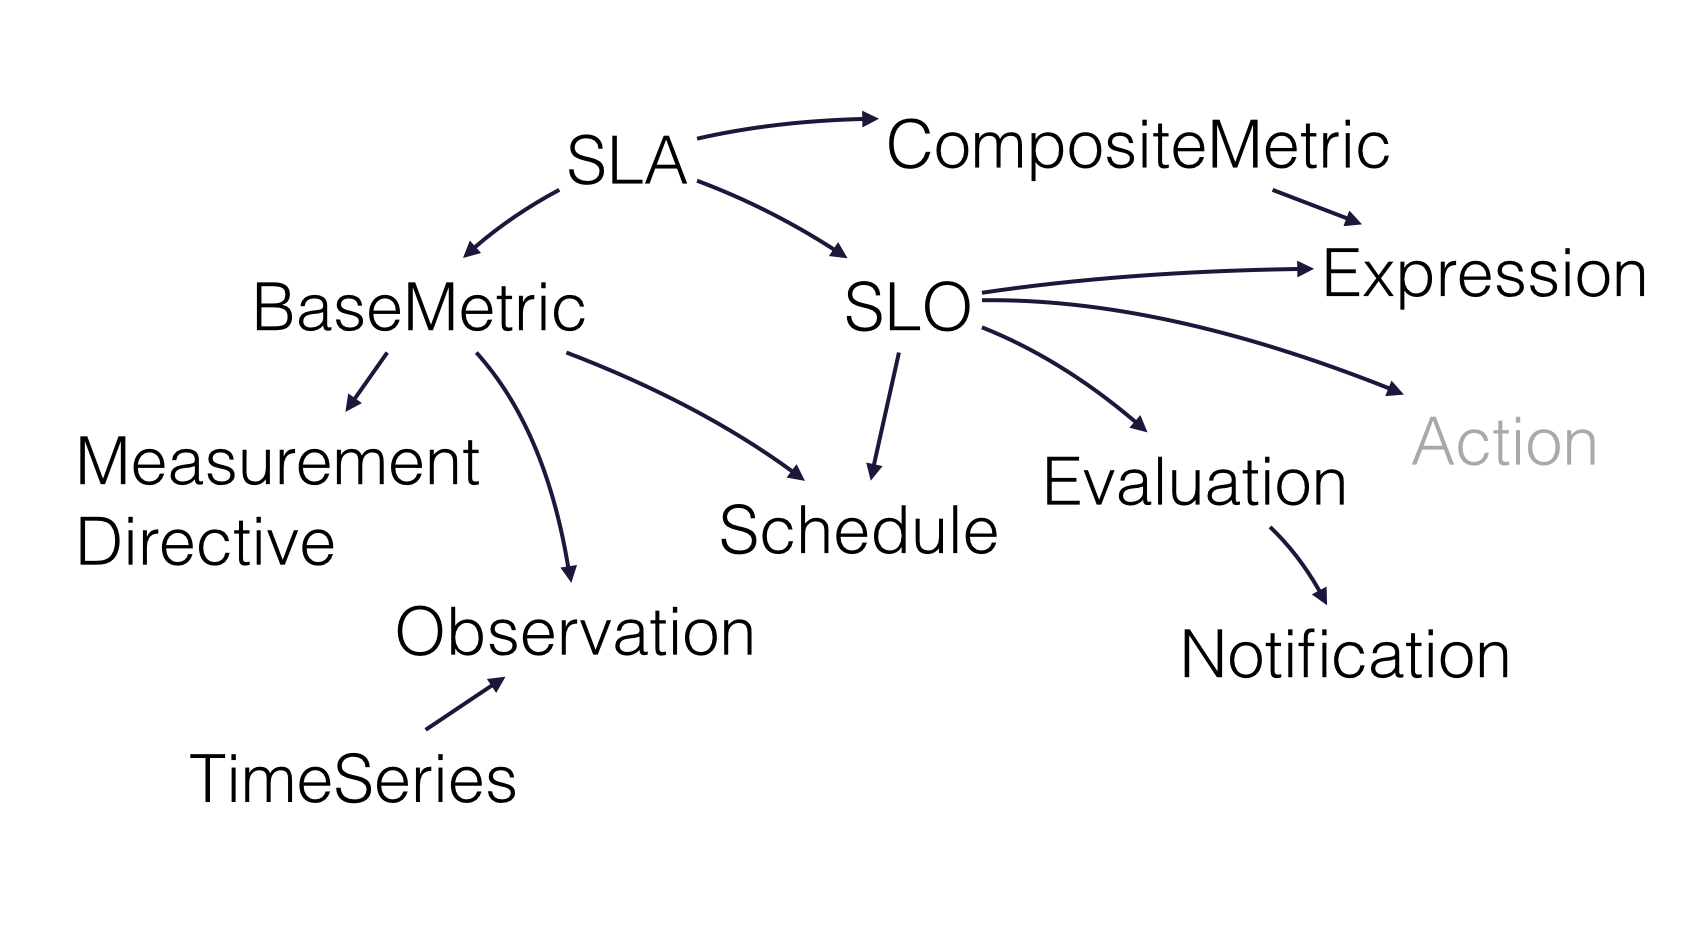
\includegraphics[width=0.5\textwidth]{pics/rslauser}
    \caption{rSLA DSL class diagram}
    \label{rSLA_diag}
\end{figure}

 rSLA supports the creation of programming blocks that express SLA context and that are necessary to run and manage rSLAs in a cloud environment. 
Listing \ref{lst} describes the rSLA vocabulary using set notation to highlight the nesting between language objects:
\begin{lstlisting}[breaklines, mathescape, firstnumber=auto, caption=rSLA vocabulary, label=lst]
SLA $\supset$ { BaseMetric+, CompositeMetric*, SLO+ }
BaseMetric $\supset$ { MeasurementDirective, Observation*, Schedule* }
CompositeMetric $\supset$ { Expression* }
SLO $\supset$ { Expression*, Action*, Evaluation*, Schedule* }
\end{lstlisting}

In the rSLA language nested relationships denote inclusive associations between objects. For example, an SLA includes base and composite metrics as 
well as SLOs. Inclusive relationships of rSLA objects do not share same multiplicity rules (listing \ref{lst}). The rSLA DSL follows the WSLA 
specification \cite{wsla} with respect to the definition of rSLA objects and of their basic attributes.

In Figure \ref{rSLA_diag} the $Notification$ and $TimeSeries$ classes do not appear in the rSLA set representation. These two classes produce objects 
that help with service level management operations like the statistical analysis of data coming from monitoring or automated notification reports on 
scheduled events of service level evaluation. Such two classes are not initially required to build and run SLA instances in a cloud environment, but 
may be required while one or more SLA management tasks are processed.



conclude that
 
\subsection{rSLA language production rules}

rSLA language constructs: elements have relationships/dependencies, there is nesting and management dependencies

production rules